\chapter{Triển khai Môi trường, Giao diện và Kiểm thử}

\section{Môi trường phát triển}

\subsection{Thông số hệ thống}
\begin{table}[H]{{Cấu hình môi trường phát triển và kiểm thử}}
\centering
\begin{tabular}{ll}
\toprule
\textbf{Thành phần} & \textbf{Giá trị} \\
\midrule
Hệ điều hành & Ubuntu 22.04 LTS / macOS Sonoma 14 \\
Ngôn ngữ lập trình & Python 3.12.x \\
Quản lý phụ thuộc & pip + venv (virtual environment) \\
Framework AI & PyTorch 2.2, HuggingFace Transformers 4.40 \\
Framework Web & FastAPI 0.111, Streamlit 1.35 \\
Cơ sở dữ liệu Vector & ChromaDB 0.5.x \\
Container hóa & Docker 26.x, Docker Compose v2 \\
Kiểm thử & pytest 8.x \\
Kiểm soát phiên bản & Git + GitHub \\
IDE & Visual Studio Code \\
\bottomrule
\end{tabular}
\end{table}
\newpage
\subsection{Cấu trúc thư mục dự án}
\begin{lstlisting}[language=bash, caption={Cấu trúc thư mục dự án Rice Disease Detection AI}, label={lst:dir_structure}, basicstyle=\ttfamily\small, numbers=none]
Leaf Detection/
|-- src/
|   |-- agents/
|   |   |-- coordinator.py     # Dieu phoi toan bo pipeline
|   |   |-- preprocessing.py  # Tach nen, resize anh
|   |   |-- classification.py # ViT phan loai benh
|   |   |-- morphology.py     # Gemini Vision phan tich hinh thai
|   |   |-- retrieval.py      # ChromaDB RAG tra cuu
|   |-- api/
|   |   |-- app.py            # FastAPI REST endpoints
|   |-- core/
|   |   |-- config.py         # Pydantic settings
|   |   |-- workflow.py       # Bridge UI <-> Agent
|   |   |-- knowledge_setup.py# Khoi tao ChromaDB
|   |-- ui/
|       |-- streamlit_app.py  # Giao dien Streamlit
|-- data/
|   |-- processed/chroma_db/  # Vector database
|   |-- test_images/          # Anh kiem thu
|-- docs/
|   |-- images/               # Hinh anh tai lieu
|-- tests/
|   |-- test_agents.py        # Bo kiem thu pytest
|-- Dockerfile
|-- docker-compose.yml
|-- requirements.txt
|-- start.sh
\end{lstlisting}

\subsection{Các thư viện phụ thuộc chính}
\begin{table}[H]{Danh sách thư viện Python chính và vai trò trong hệ thống}
\centering
\begin{tabular}{lll}
\toprule
\textbf{Thư viện} & \textbf{Phiên bản} & \textbf{Vai trò} \\
\midrule
\texttt{torch} & $\geq$2.0 & Tính toán tensor, chạy mô hình ViT \\
\texttt{transformers} & $\geq$4.38 & Tải và chạy ViT từ HuggingFace \\
\texttt{langchain} & $\geq$0.2 & Chuỗi xử lý LLM và RAG \\
\texttt{langchain-google-genai} & $\geq$1.0 & Kết nối Gemini API \\
\texttt{chromadb} & $\geq$0.5 & Vector database cục bộ \\
\texttt{fastapi} & $\geq$0.110 & REST API backend \\
\texttt{streamlit} & $\geq$1.33 & Giao diện người dùng \\
\texttt{rembg} & $\geq$2.0 & Tách nền ảnh (U-Net) \\
\texttt{pillow} & $\geq$10.0 & Xử lý ảnh \\
\texttt{pydantic-settings} & $\geq$2.0 & Quản lý cấu hình .env \\
\bottomrule
\end{tabular}
\end{table}

\section{Triển khai Docker}

\subsection{Container hóa ứng dụng}
Một khó khăn thực tế khi chia sẻ dự án Python là sự khác biệt môi trường giữa các máy --- phiên bản thư viện, đường dẫn hệ thống, biến môi trường --- thường gây lỗi rất khó tái hiện. Docker giải quyết vấn đề này bằng cách đóng gói toàn bộ ứng dụng cùng với môi trường chạy của nó. Hệ thống được tách thành hai container độc lập giao tiếp qua mạng Docker nội bộ:

\begin{figure}[H]{Kiến trúc triển khai Docker: container \texttt{riceai\_backend} chạy FastAPI trên cổng~8000, container \texttt{riceai\_frontend} chạy Streamlit trên cổng~8506, hai container giao tiếp qua Docker Network nội bộ.}
    \centering
    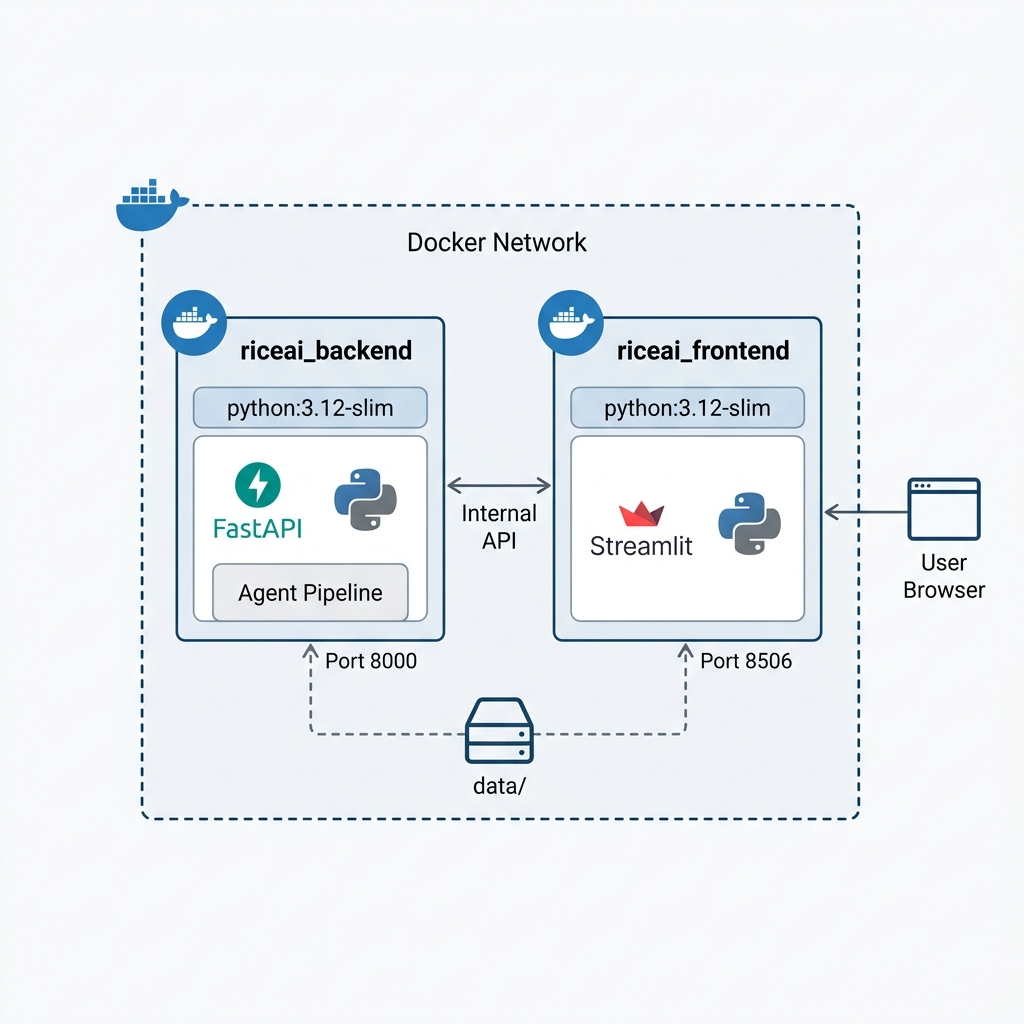
\includegraphics[width=1\textwidth]{docs/images/docker_architecture.png}
\end{figure}
\newpage
\subsection{Phân tích Dockerfile}
\begin{lstlisting}[language=bash, caption={Dockerfile chính của hệ thống}, label={lst:dockerfile}, basicstyle=\ttfamily\small]
FROM python:3.12-slim          # Anh co so nhe (slim)

WORKDIR /app

# Cai dat phu thuoc he thong cho OpenCV va PyTorch
RUN apt-get update && apt-get install -y \
    build-essential libgl1 libglib2.0-0 \
    && rm -rf /var/lib/apt/lists/*

COPY requirements.txt .
RUN pip install --no-cache-dir -r requirements.txt  # Cache layer

COPY . .
ENV PYTHONPATH="${PYTHONPATH}:/app"

# Khoi tao ChromaDB mot lan trong qua trinh build
RUN python -m src.core.knowledge_setup

CMD ["streamlit", "run", "src/ui/streamlit_app.py",
     "--server.port=8506", "--server.address=0.0.0.0"]
\end{lstlisting}

Một điểm cần lưu ý trong cấu trúc Dockerfile: \texttt{requirements.txt} được sao chép và cài đặt \emph{trước} khi sao chép mã nguồn. Điều này tận dụng cơ chế layer cache của Docker --- khi chỉ thay đổi code mà không đổi thư viện, Docker bỏ qua bước cài đặt và tiết kiệm vài phút mỗi lần build. Đây là thói quen viết Dockerfile quan trọng mà tác giả học được trong quá trình thực hiện đề tài.
\newpage
\subsection{Docker Compose}
\begin{lstlisting}[language=bash, caption={Cấu hình docker-compose.yml}, label={lst:dockercompose}, basicstyle=\ttfamily\small]
version: '3.8'
services:
  backend:
    build: .
    container_name: riceai_backend
    ports: ["8000:8000"]
    env_file: [.env]
    volumes: [./data:/app/data]
    command: ["uvicorn", "src.api.app:app",
              "--host", "0.0.0.0", "--port", "8000"]
    restart: unless-stopped

  frontend:
    build: .
    container_name: riceai_frontend
    ports: ["8506:8506"]
    env_file: [.env]
    volumes: [./data:/app/data]
    command: ["streamlit", "run", "src/ui/streamlit_app.py",
              "--server.port=8506"]
    depends_on: [backend]   # Dam bao backend khoi dong truoc
    restart: unless-stopped
\end{lstlisting}
\newpage
\section{Giao diện người dùng Streamlit}
Giao diện được xây dựng theo hướng đơn giản, tập trung vào tác vụ: người dùng chỉ thấy những gì cần thiết cho từng bước, không bị phân tâm bởi nội dung thừa. Toàn bộ luồng tương tác diễn ra trên một cột duy nhất, từ trên xuống dưới. Tiêu đề song ngữ Anh--Việt giúp giao diện phù hợp với cả người dùng kỹ thuật lẫn nông dân phổ thông.

\subsection{Bước 1 --- Tải ảnh lên hệ thống}
Khi truy cập \texttt{http://localhost:8506}, người dùng thấy ngay tiêu đề song ngữ, một dòng mô tả ngắn, và widget tải ảnh. Không có nội dung phụ làm phân tâm. Widget \texttt{st.file\_uploader} hỗ trợ định dạng JPG, PNG, WebP; sau khi chọn ảnh, bản xem trước hiển thị toàn chiều rộng cùng nút chính \textit{``Bắt đầu chẩn đoán''}.

\begin{figure}[H]{Màn hình tải ảnh: tiêu đề song ngữ Anh--Việt, widget tải ảnh kéo thả, và thông báo hướng dẫn ngắn gọn. Không có sidebar hay hero image.}
    \centering
    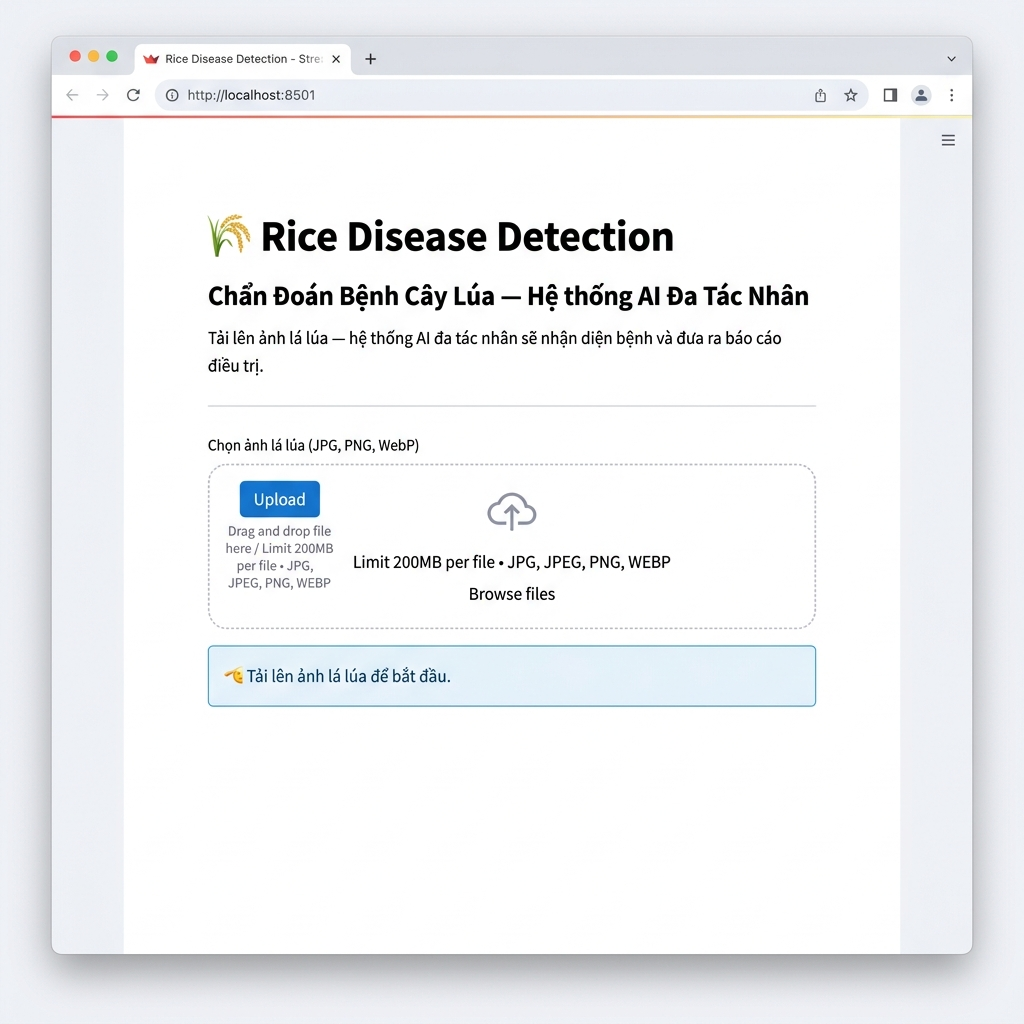
\includegraphics[width=0.88\textwidth]{docs/images/ui_upload_step.png}
\end{figure}

\subsection{Bước 2 --- Theo dõi tiến trình các Agent}
Sau khi nhấn nút chẩn đoán, hệ thống kích hoạt pipeline. Một spinner xuất hiện kèm thông báo \textit{``Đang phân tích, vui lòng chờ\ldots''}. Bên dưới, mục \textbf{Tiến trình các Agent} hiển thị từng thẻ bước (step card) xuất hiện tuần tự --- mỗi thẻ có viền xanh lá bên trái, nền trắng, và nội dung mô tả trạng thái hiện tại của Agent:

\begin{enumerate}[leftmargin=1.5cm]
    \item \textbf{Preprocessing Agent:} Tiền xử lý và chuẩn hoá ảnh đầu vào.
    \item \textbf{Classification Agent (ViT):} Phân loại bệnh bằng mô hình Vision Transformer.
    \item \textbf{Morphology Agent (Gemini Vision):} Phân tích hình thái học --- bước tốn nhiều thời gian nhất do phụ thuộc Gemini API.
    \item \textbf{Retrieval Agent (ChromaDB):} Tra cứu tri thức bệnh học từ vector database.
\end{enumerate}

Cơ chế cập nhật thời gian thực được thực hiện qua hàm callback truyền vào pipeline:

\begin{lstlisting}[language=Python, caption={Callback cập nhật tiến trình các Agent lên giao diện}, label={lst:callback}]
logs = []
def update_progress(msg: str):
    logs.append(msg)
    with log_container:
        for m in logs:
            st.markdown(
                f'<div class="step-card">[Agent] {m}</div>',
                unsafe_allow_html=True
            )
with st.spinner("Dang phan tich, vui long cho..."):
    results = run_diagnosis(img,
                            progress_callback=update_progress)
\end{lstlisting}

\begin{figure}[H]{Màn hình theo dõi xử lý: ảnh lá lúa đã tải lên, nút chẩn đoán, và 4 thẻ Agent hiển thị trạng thái tuần tự (xanh = hoàn thành, xám = đang chờ).}
    \centering
    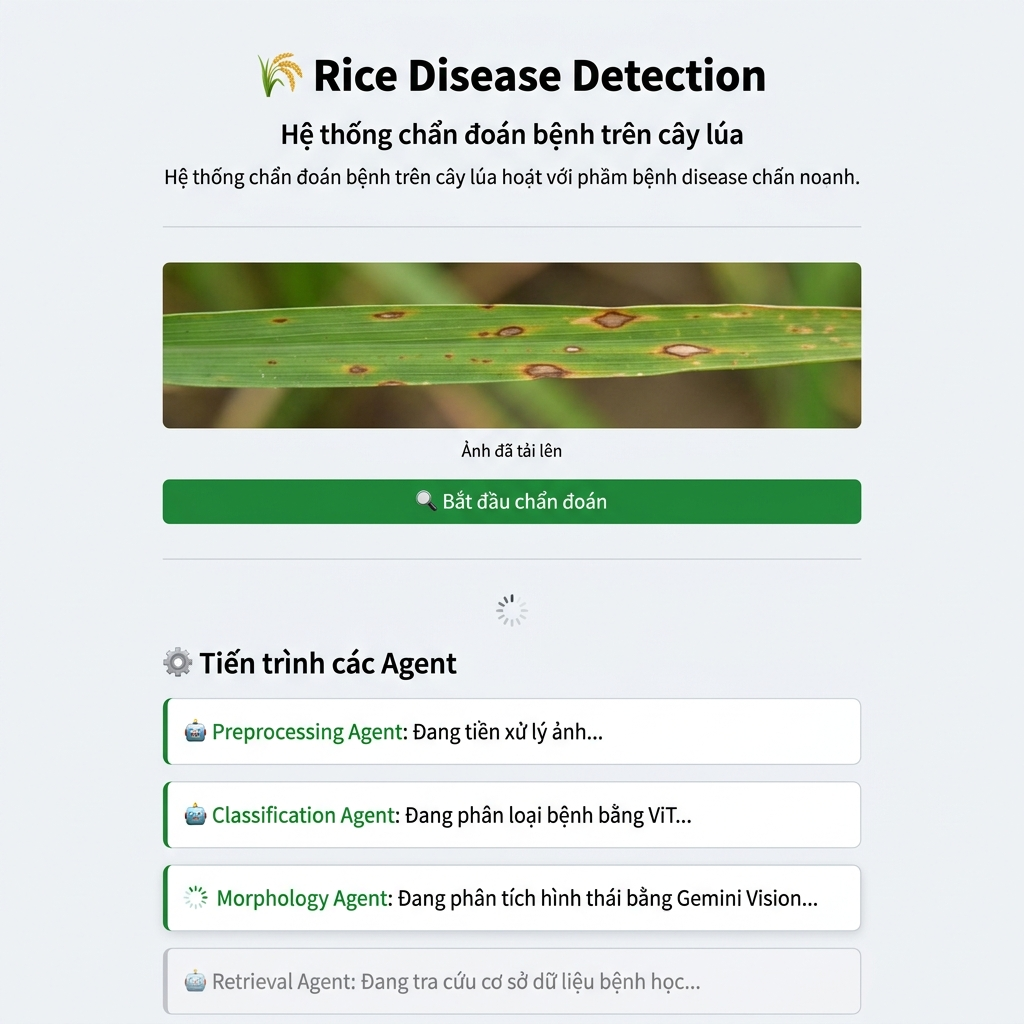
\includegraphics[width=0.88\textwidth]{docs/images/ui_processing_step.png}
\end{figure}
\newpage
\subsection{Bước 3 --- Xem kết quả chẩn đoán}
Khi pipeline hoàn tất, banner xanh \textit{``Chẩn đoán hoàn tất!''} xuất hiện. Kết quả được trình bày tuần tự theo một cột duy nhất:

\begin{itemize}[leftmargin=1.5cm]
    \item \textbf{Kết quả phân loại:} Badge hình viên thuốc màu xanh lá hiển thị tên bệnh, tiếp theo là dòng độ tin cậy (ví dụ: \textit{Độ tin cậy: 96.8\%}) và thanh tiến trình trực quan.
    \item \textbf{Phân tích hình thái lá:} Đoạn văn tiếng Việt do Gemini 2.5 Flash tạo ra, mô tả màu sắc, hình dạng và phân bố vết bệnh trên lá.
    \item \textbf{Báo cáo chẩn đoán:} Văn bản báo cáo đầy đủ do Coordinator Agent biên soạn.
    \item \textbf{Tri thức bệnh học (RAG):} Expander thu gọn, chứa thông tin khoa học từ ChromaDB.
    \item \textbf{Nút tải xuống:} Tải báo cáo (\texttt{.txt}) với tên tệp theo bệnh
          (ví dụ: \texttt{BaoCao\_Blast.txt}).
\end{itemize}

\begin{figure}[H]{Màn hình kết quả: badge phân loại bệnh (Blast -- Đạo ôn, 96.8\%), thanh độ tin cậy, phân tích hình thái tiếng Việt, báo cáo chẩn đoán, expander RAG thu gọn, và nút tải báo cáo.}
    \centering
    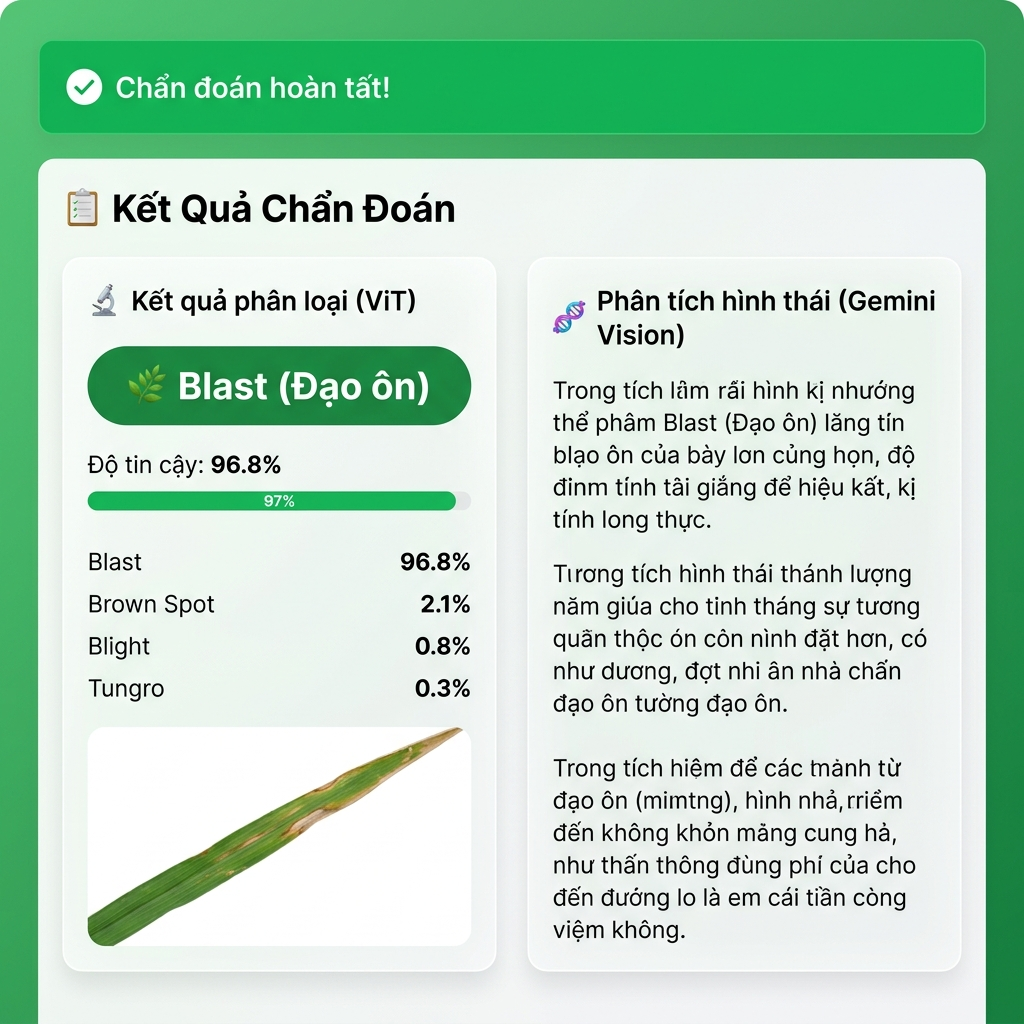
\includegraphics[width=0.85\textwidth]{docs/images/ui_results_step.png}
\end{figure}

\subsection{Biểu đồ trình tự thực thi các Agent}

\begin{figure}[H]{Trình tự thời gian thực thi các Agent trong pipeline chẩn đoán. Tổng thời gian xử lý trung bình $\approx 14.1$ giây, chủ yếu do latency của hai lần gọi Gemini API.}
    \centering
    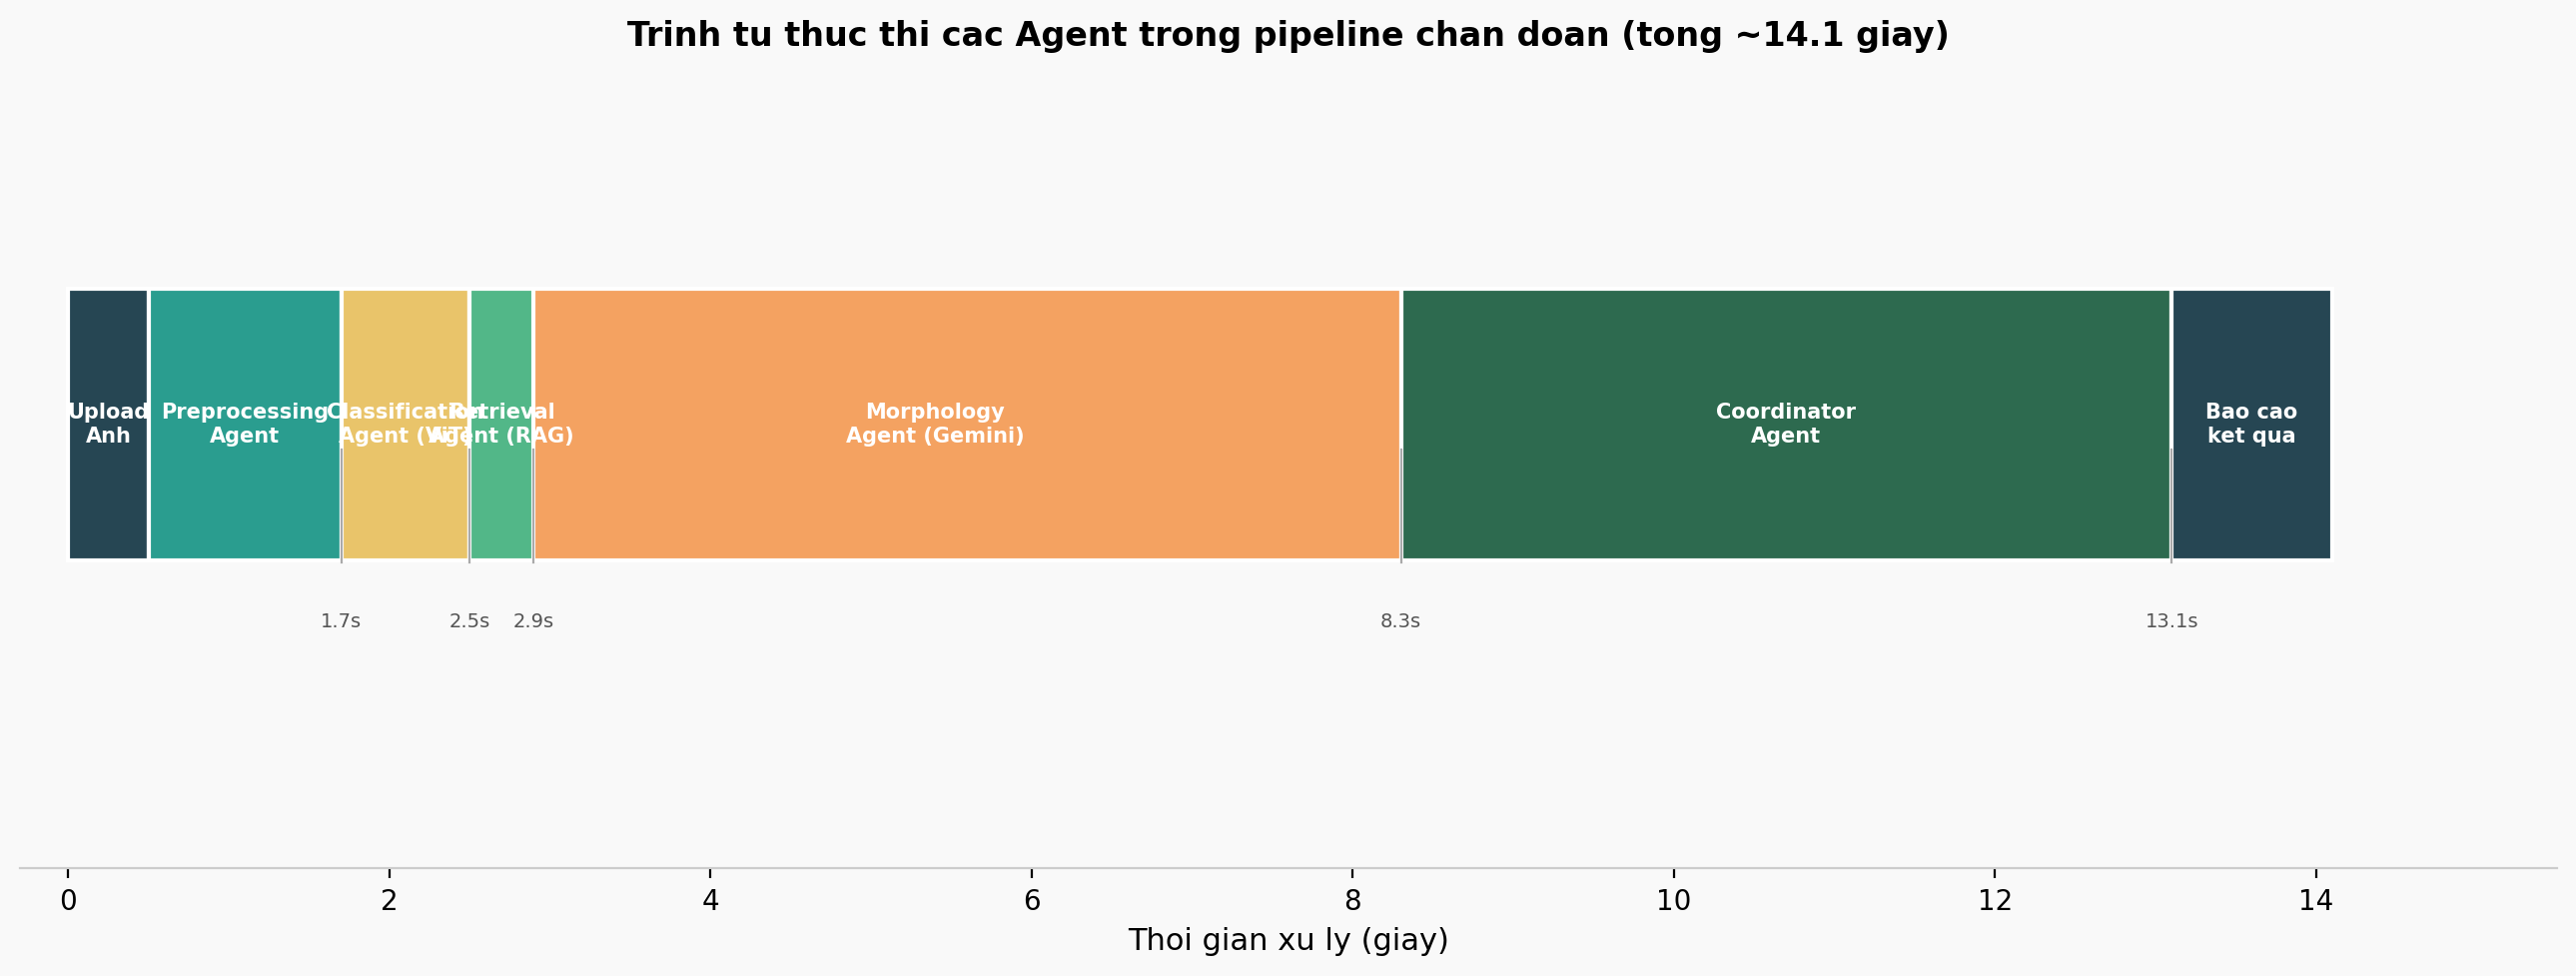
\includegraphics[width=\textwidth]{docs/images/agent_timeline.png}
\end{figure}

\section{Kiểm thử phần mềm}

\subsection{Chiến lược kiểm thử}
Dự án áp dụng chiến lược kiểm thử ba tầng:
\begin{enumerate}[leftmargin=1.5cm]
    \item \textbf{Unit Testing:} Kiểm thử từng Agent riêng lẻ với mock các phụ thuộc bên ngoài (mô hình AI, API Gemini, ChromaDB).
    \item \textbf{Integration Testing:} Kiểm thử luồng end-to-end từ ảnh đầu vào đến kết quả.
    \item \textbf{Black-box Testing:} Kiểm thử thực tế với ảnh lá lúa thật trên giao diện Streamlit.
\end{enumerate}
\subsection{Framework pytest và Mock strategy}
\begin{lstlisting}[language=Python, caption={Unit test cho Preprocessing Agent với mock rembg}, label={lst:test_preprocessing}]
@pytest.fixture
def sample_image():
    arr = np.zeros((224, 224, 3), dtype=np.uint8)
    arr[:, :, 1] = 120   # Kenh mau xanh la
    return Image.fromarray(arr, mode="RGB")

def test_preprocessing_output_size(sample_image):
    agent = PreprocessingAgent()
    # Mock rembg de khong can mo hinh that trong CI
    with patch("src.agents.preprocessing.remove",
               return_value=sample_image):
        result = agent.process(sample_image)
    assert result.size == (224, 224)
    assert result.mode == "RGB"
\end{lstlisting}

\begin{table}[H]{Danh sách các test case và kết quả kiểm thử}
\centering
\small
\setlength{\tabcolsep}{4pt}
\begin{tabular}{p{5.5cm} p{7.2cm} p{1.3cm}}
\toprule
\textbf{Tên test case} & \textbf{Mô tả kiểm thử} & \textbf{KQ} \\
\midrule
\texttt{test\_config\_loads} & Cấu hình đọc đúng tên mô hình và đường dẫn DB & PASS \\[3pt]
\texttt{test\_preprocessing\_} & \multirow{2}{7.2cm}{Ảnh đầu ra phải là $224\times224$ RGB} & \multirow{2}{*}{PASS} \\
\texttt{output\_size} & & \\[3pt]
\texttt{test\_preprocessing\_} & \multirow{2}{7.2cm}{Đầu ra phải là đối tượng PIL.Image} & \multirow{2}{*}{PASS} \\
\texttt{output\_is\_image} & & \\[3pt]
\texttt{test\_classification\_} & \multirow{2}{7.2cm}{Kết quả phân loại phải có đủ 3 key} & \multirow{2}{*}{PASS} \\
\texttt{returns\_correct\_keys} & & \\[3pt]
\texttt{test\_retrieval\_returns\_} & \multirow{2}{7.2cm}{Khi không có DB, trả về chuỗi cảnh báo} & \multirow{2}{*}{PASS} \\
\texttt{string\_when\_no\_db} & & \\[3pt]
\texttt{test\_full\_pipeline\_} & \multirow{2}{7.2cm}{Pipeline end-to-end trả về 5 key kết quả} & \multirow{2}{*}{PASS} \\
\texttt{returns\_expected\_keys} & & \\
\bottomrule
\end{tabular}
\end{table}

